%!TEX root = ../thesis.tex
% ******************************* Thesis Appendix A ****************************

\begin{figure}[htbp!] 
\centering    
    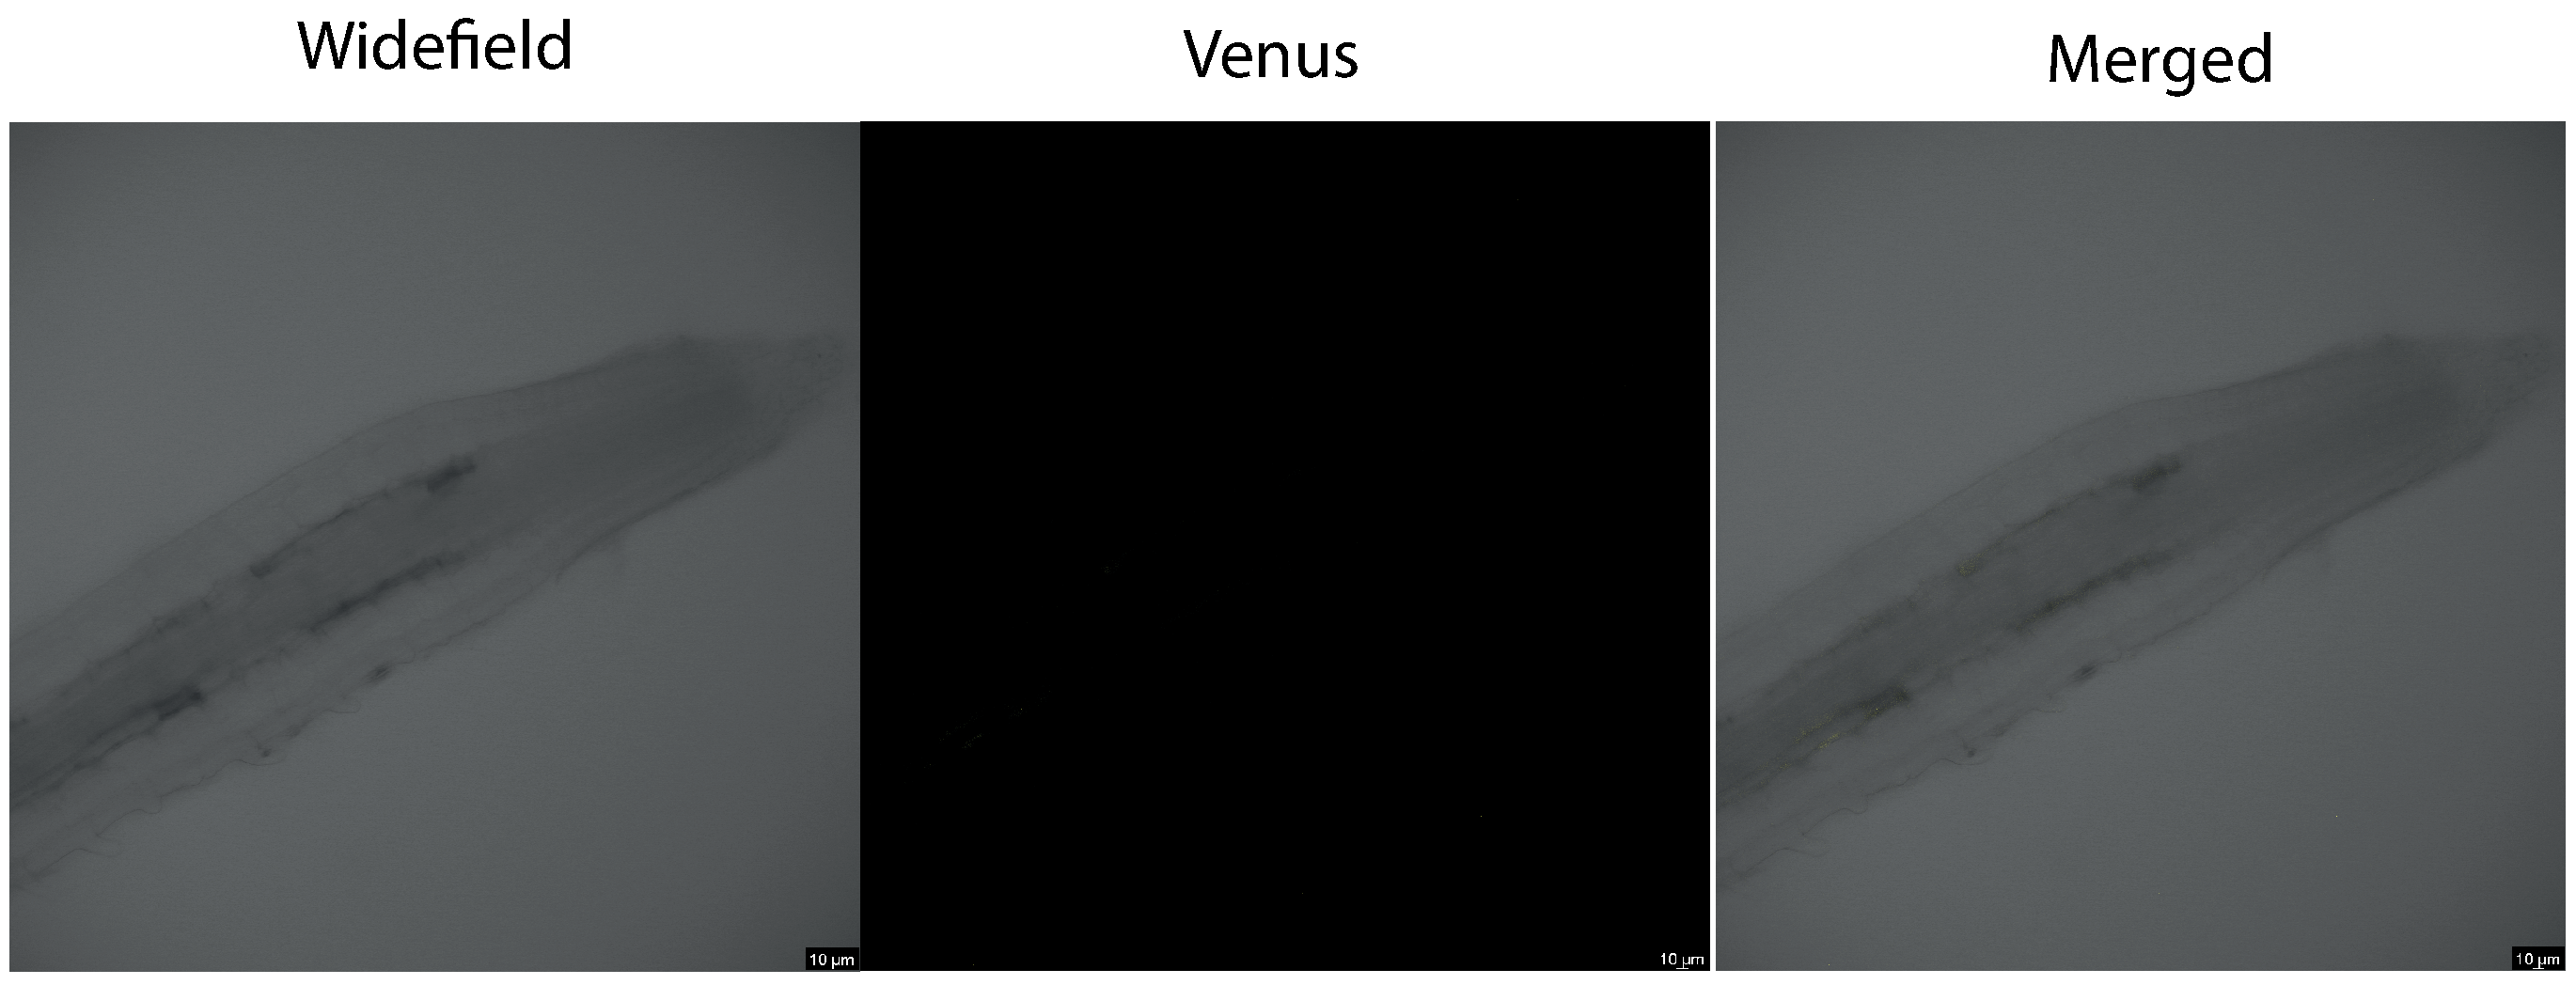
\includegraphics[width=1\textwidth]{Chapter2/Figs/Supps/FigureS1_CLSY3_Root_tip_neg.pdf}
\caption{\textbf{pCLSY3::CLSY3-Venus is not expressed in the root tip}}
\label{fig:clsy3_root}
\captionsetup{font=small}
    \caption*{Scale bar 10 $\mu$m.}
\end{figure}

\begin{figure}[htbp!] 
\centering    
    \includegraphics[width=1\textwidth]{Chapter2/Figs/Supps/FigureS2_CLSY1_2_Pollen.pdf}
\caption{\textbf{CLSY1 and CLSY2 are not specifically expressed in the pollen}}
\label{fig:clsy1_2_pollen}
\captionsetup{font=small}
    \caption*{DAPI (blue, second row) staining of pCLSY1::CLY1-eGFP (first row) and pCLSY2::CLY2-eGFP (second row) showing no expression of CLSYs (third column, GFP, green) in mature pollen. Scale bar 10 $\mu$m.}
\end{figure}

\begin{figure}[htbp!] 
\centering    
    \includegraphics[width=1\textwidth]{Chapter2/Figs/Supps/FigureS3_Pol4_Pol5_roots.pdf}
\caption{\textbf{pNRPD1::NRPD1-eGFP and pNRPE1::NRPE1-eGFP are strongly expressed in the root}}
\label{fig:Pol4_5_roots}
\captionsetup{font=small}
    \caption*{eGFP (green, white arrows) nuclear signal of NRPD1 (first row) and NRPE1 (second row) in the root tip of \textit{Arabidopsis}. Scale bar 10 $\mu$m.}
\end{figure}

\begin{figure}[htbp!] 
\centering    
    \includegraphics[width=1\textwidth]{Chapter2/Figs/Supps/FigureS4_Pol4_germline_no_expression.pdf}
\caption{\textbf{pNRPD1 is not consistently expressed in germline tissues}}
\label{fig:Pol4_germ_no_expression}
\captionsetup{font=small}
    \caption*{eGFP (green) DAPI (blue). Scale bar 10 $\mu$m.}
\end{figure}

\begin{figure}[htbp!] 
\centering    
    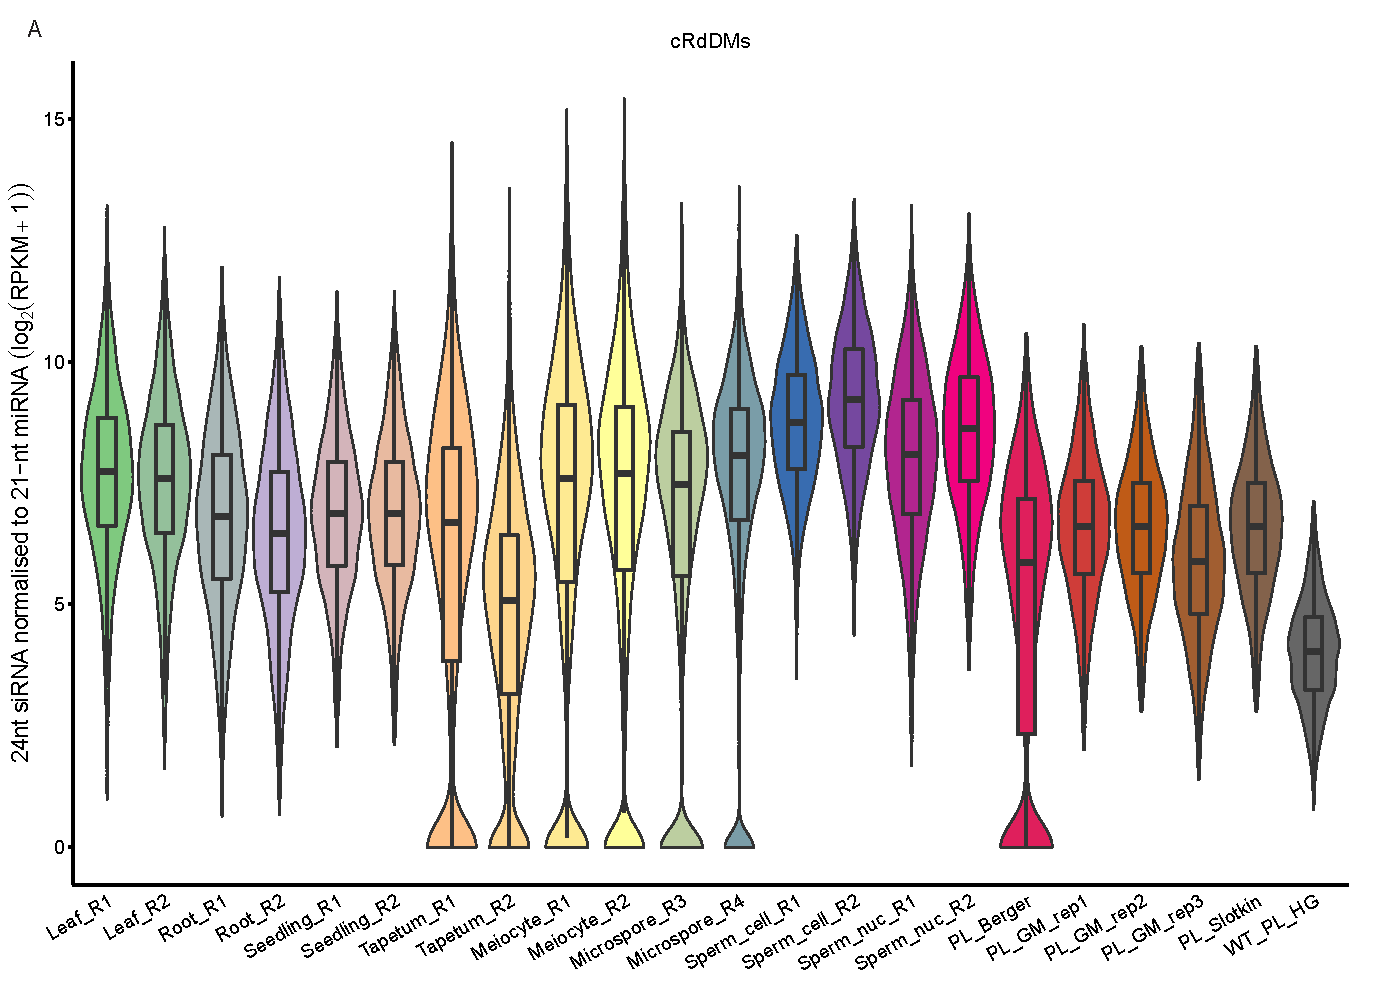
\includegraphics[width=1\textwidth]{Chapter2/Figs/Supps/FigureS7_miRNA_norm.pdf}
\caption{\textbf{}}
\label{fig:miRNA_norm}
\captionsetup{font=small}
    \caption*{}
\end{figure}

\begin{figure}[htbp!] 
\centering    
    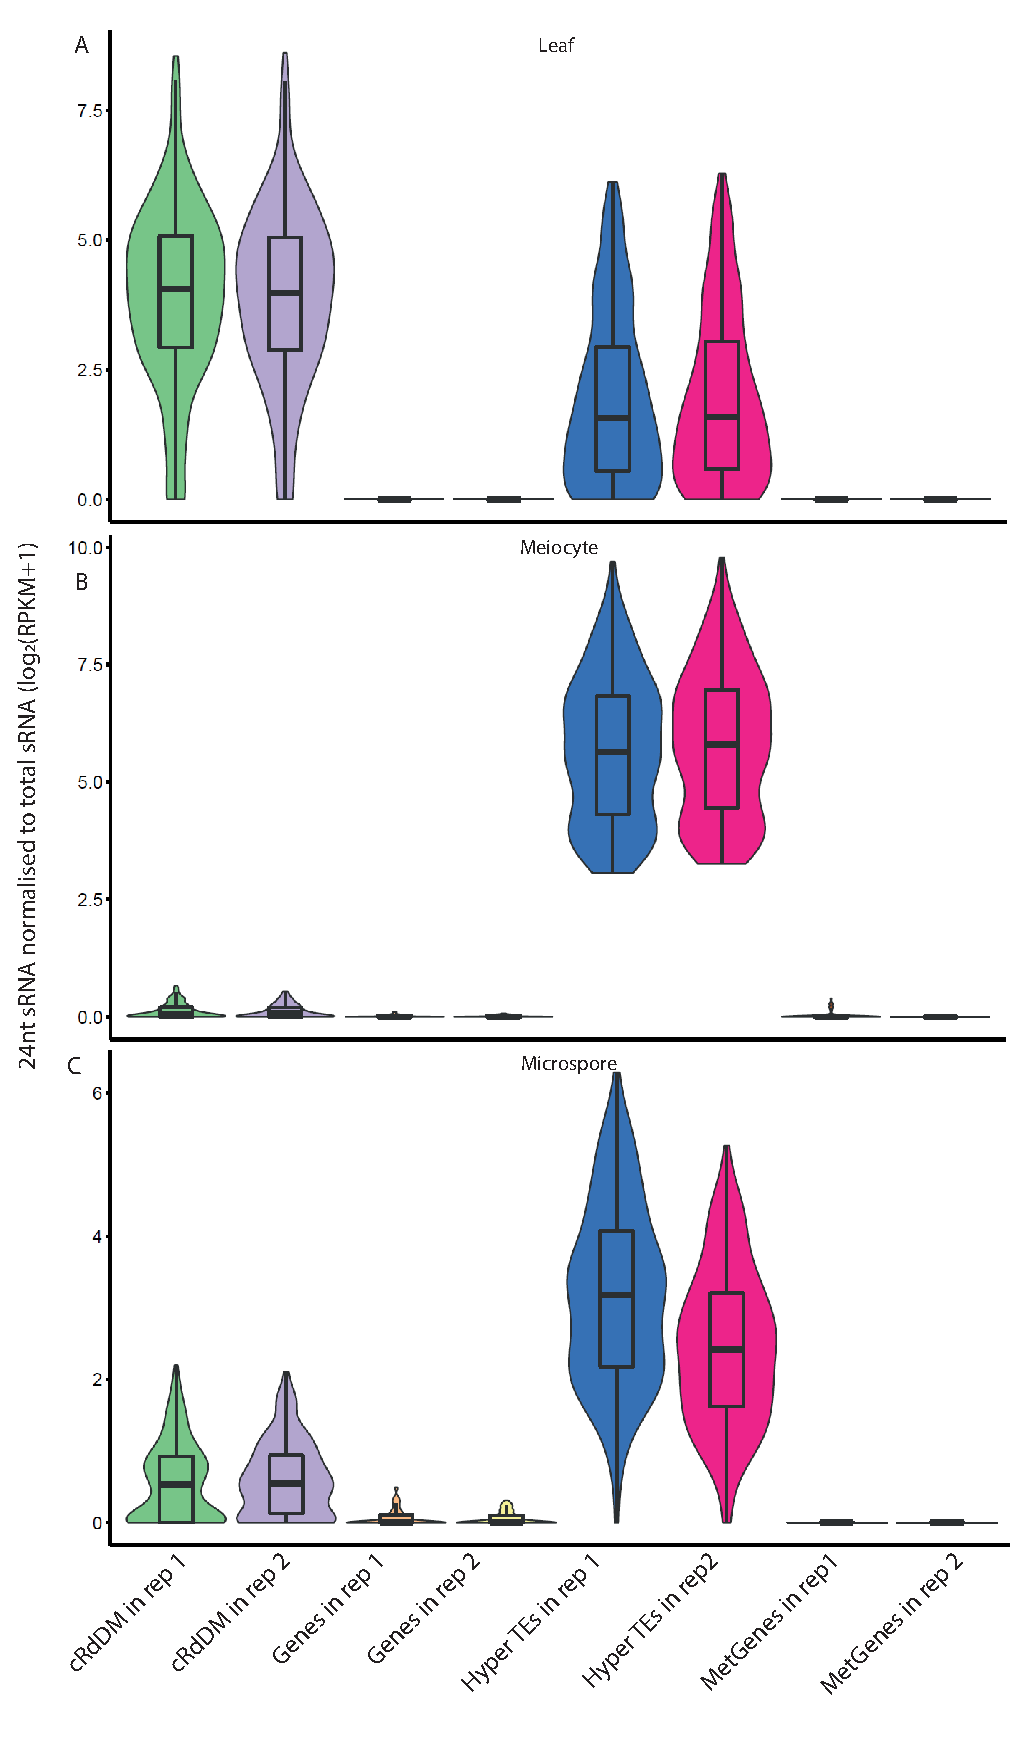
\includegraphics[width=0.8\textwidth]{Chapter2/Figs/Supps/FigureS8_boxplots_meiocyte_microspore.pdf}
\caption{\textbf{}}
\label{fig:boxplot-MCMS}
\captionsetup{font=small}
    \caption*{}
\end{figure}

\begin{figure}[htbp!] 
\centering    
    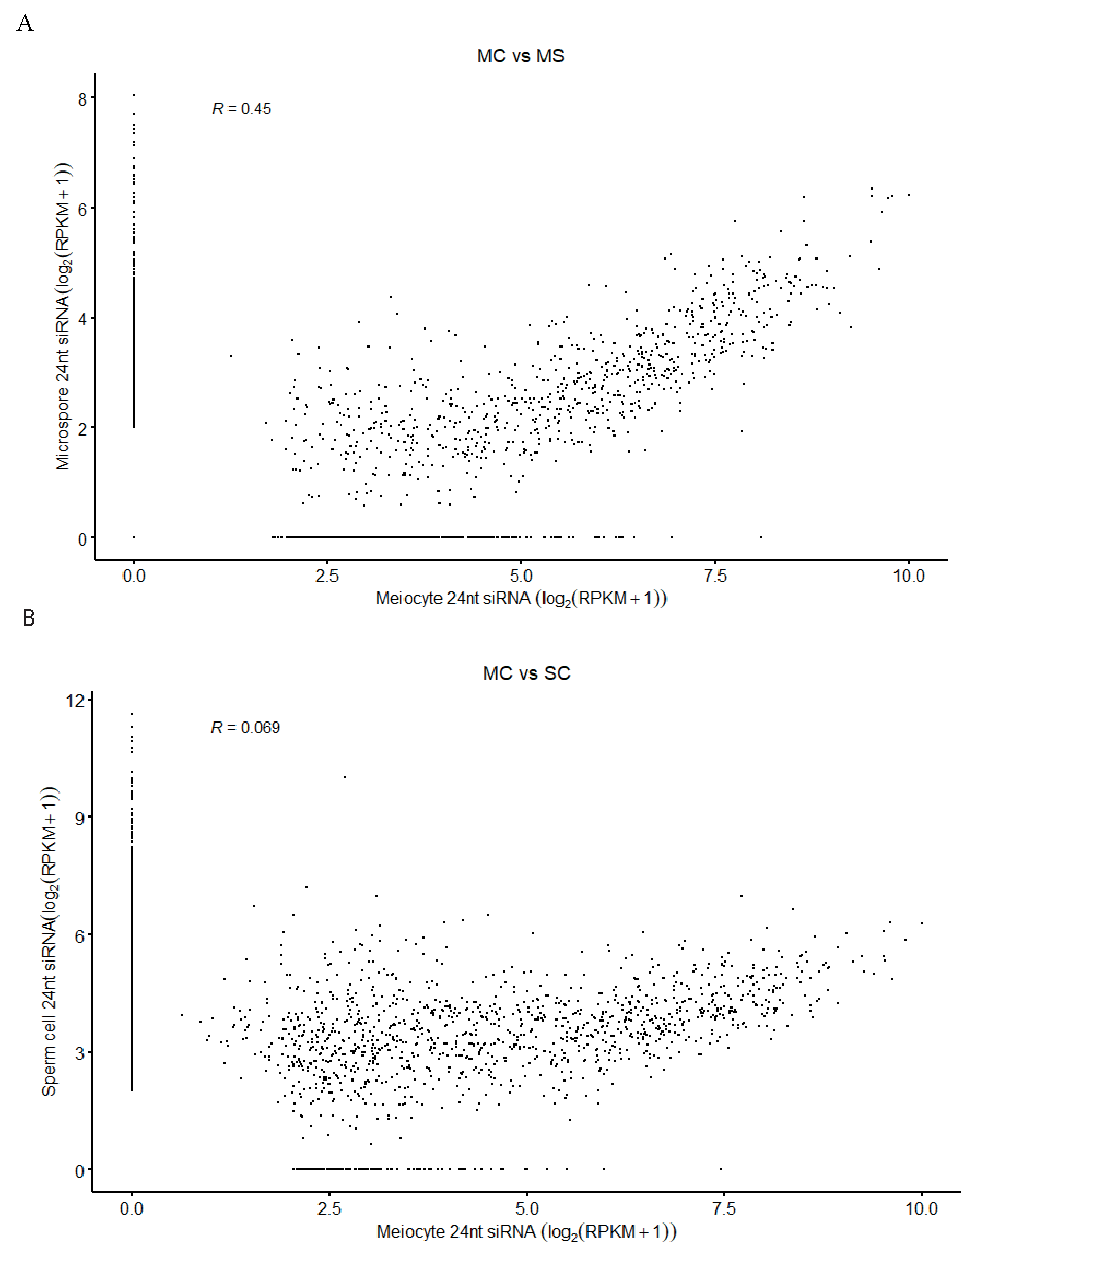
\includegraphics[width=1\textwidth]{Chapter2/Figs/Supps/FigureS5_MSSCMC_scatters.pdf}
\caption{\textbf{}}
\label{fig:MSSVMC_scatters}
\captionsetup{font=small}
    \caption*{}
\end{figure}

\begin{figure}[htbp!] 
\centering    
    \includegraphics[width=1\textwidth]{Chapter2/Figs/Supps/FigureS6_scatterplots.pdf}
\caption{\textbf{}}
\label{fig:clsysingle_cRdDM_scatters}
\captionsetup{font=small}
    \caption*{}
\end{figure}

\begin{figure}[htbp!] 
\centering    
    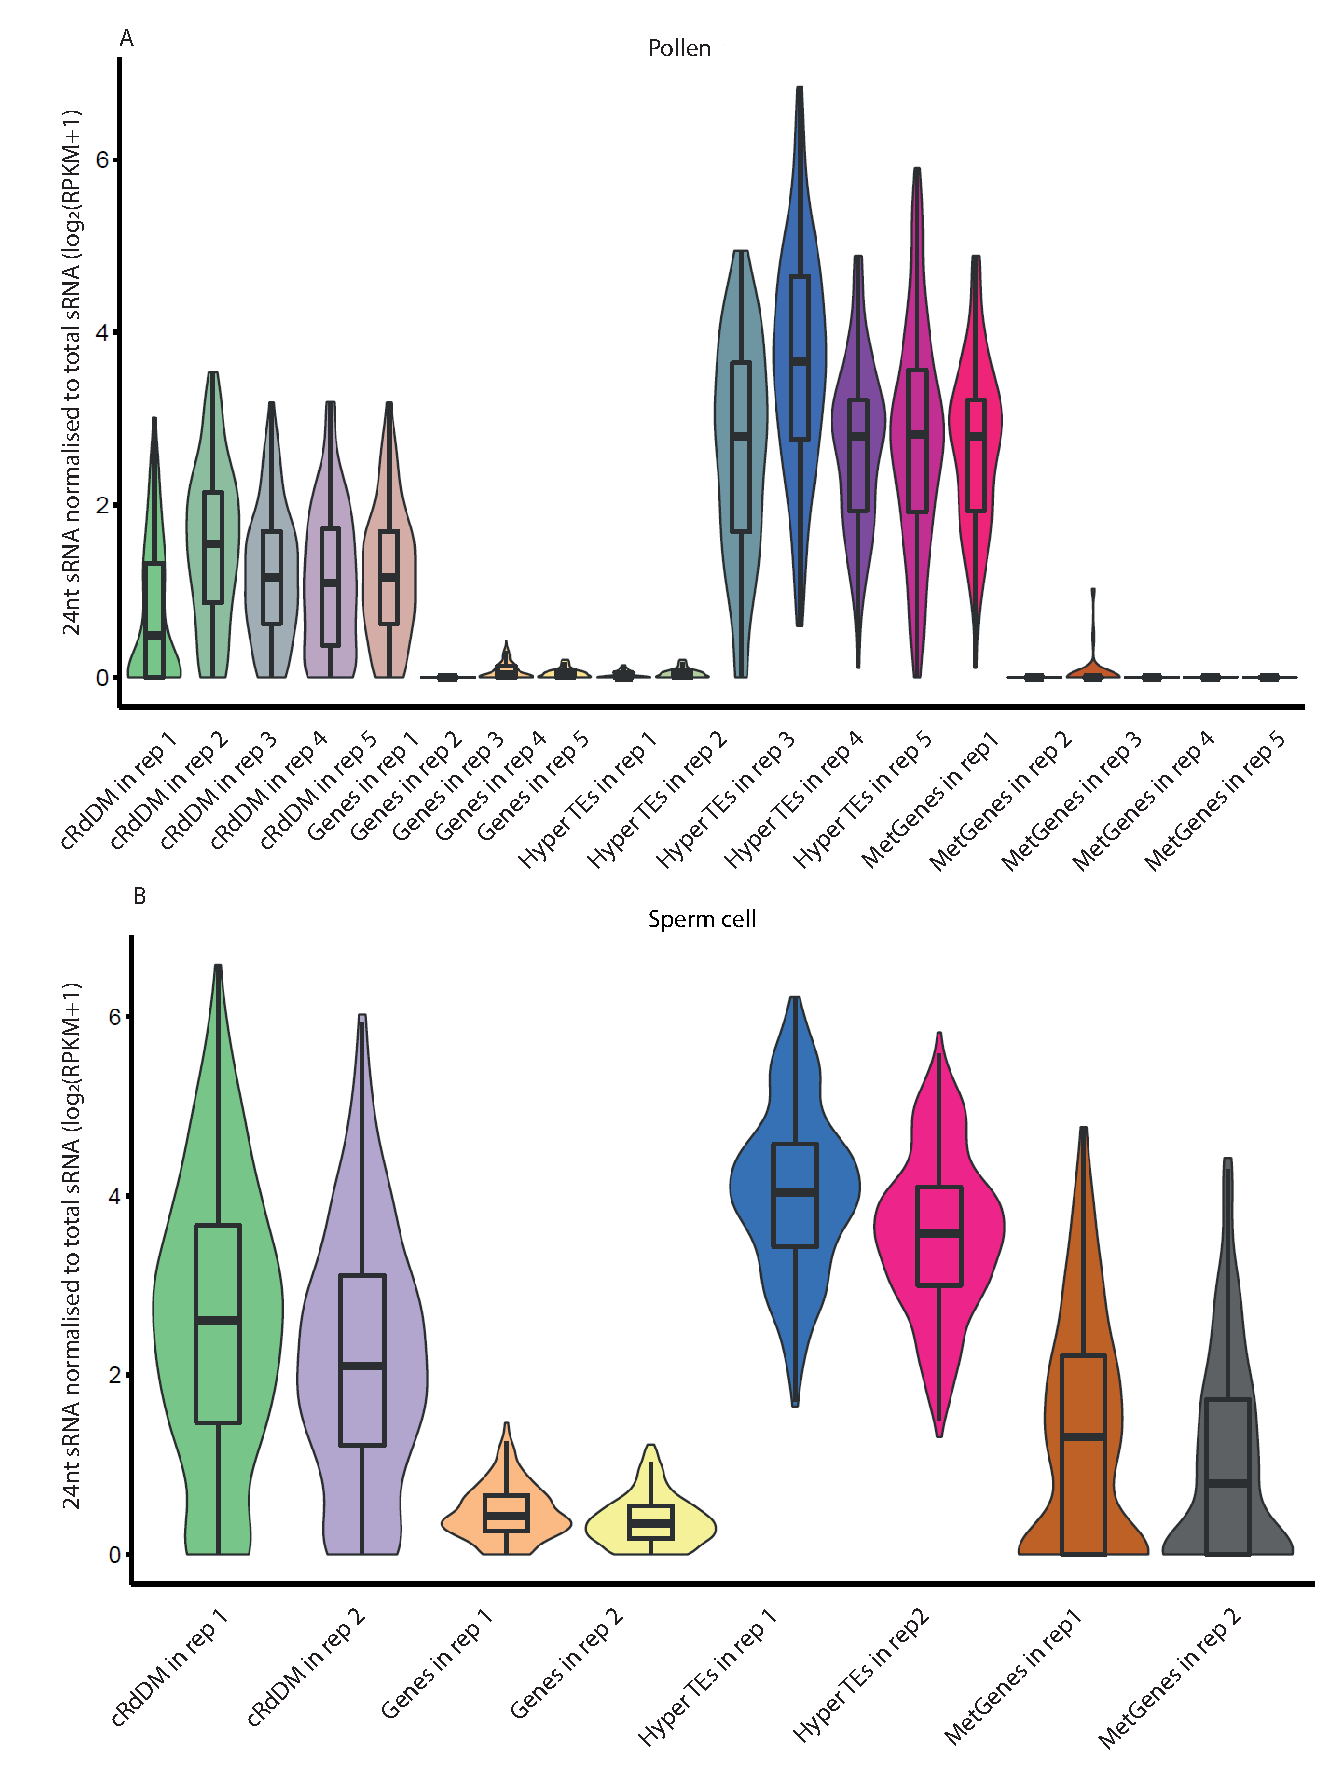
\includegraphics[width=1\textwidth]{Chapter2/Figs/Supps/FigureS9_sperm_pollen_boxplots.pdf}
\caption{\textbf{}}
\label{fig:boxplot-SCPL}
\captionsetup{font=small}
    \caption*{}
\end{figure}
